\documentclass[10pt]{article}
%#%% HEDAER FOR KERAS REPORTS %%%
\usepackage[T1]{fontenc}
\usepackage[headheight=1.5cm,top=3cm,left=2cm,right=2cm]{geometry}
\usepackage{amsfonts}
\usepackage{helvet}
\usepackage{longtable}
\usepackage{hyperref}
\usepackage{graphicx}

\usepackage{caption}
\usepackage{subcaption}

\usepackage[dvipsnames]{xcolor}
\usepackage{float}
\usepackage{fancyhdr}
\usepackage{multirow}
\usepackage{array}
\newcolumntype{L}[1]{>{\raggedright\let\newline\\\arraybackslash\hspace{0pt}}m{#1}}
\newcolumntype{C}[1]{>{\centering\let\newline\\\arraybackslash\hspace{0pt}}m{#1}}
\newcolumntype{R}[1]{>{\raggedleft\let\newline\\\arraybackslash\hspace{0pt}}m{#1}}

%# For the No. sign
\usepackage{stackengine}
\newcommand\No[1][.13ex]{%
  \setbox0=\hbox{\scalebox{.7}{o}}%
  \setbox2=\hbox{N}%
  N\kern-.05em\stackengine{\dimexpr\ht0-\ht2+#1}{\belowbaseline[-\ht2]{\copy0}}%
    {\rule[-.13ex]{.7\wd0}{.13ex}}%
    {U}{c}{F}{F}{L}%
}

%# for plots
\usepackage{pbox}
\usepackage{pgf,tikz,pgfplots}
\pgfplotsset{compat=1.15}
\usepackage{mathrsfs}
\usetikzlibrary{arrows}
\definecolor{qqqqff}{rgb}{0,0,1}
\definecolor{ffqqqq}{rgb}{1,0,0}

\usepackage{color, colortbl}
\usetikzlibrary{arrows,positioning}
\renewcommand{\familydefault}{\sfdefault}
\setlength{\parindent}{0pt}
\setlength{\parskip}{10pt}
\pagestyle{fancy}
\renewcommand{\headrulewidth}{0.0pt}
\fancyhf{}


\renewcommand{\labelenumii}{\theenumii}
\renewcommand{\theenumii}{\theenumi.\arabic{enumii}.}
\usepackage{enumitem}

\usepackage{listings}

\newcommand{\dev}[1]{{\sc #1}}

\usepackage{siunitx}
\usepackage{tabularx}
\newcolumntype{L}[1]{>{\raggedright\arraybackslash}p{#1}}
\newcolumntype{C}[1]{>{\centering\arraybackslash}p{#1}}
\newcolumntype{R}[1]{>{\raggedleft\arraybackslash}p{#1}}



\newcommand{\doctitle}{TITLE}
\newcommand{\docauthor}{AUTHOR}

\title{\doctitle}
\author{\docauthor}


\definecolor{InputLayer}{RGB}{44, 189, 201} %light blue

\definecolor{Conv2D}{RGB}{235, 101, 52} % orange/red
\definecolor{Dense}{RGB}{235, 52, 55} %red
\definecolor{BatchNormalization}{RGB}{235, 52, 140} %pink

\definecolor{Activation}{RGB}{92, 52, 235} %blue
\definecolor{Dropout}{RGB}{50, 81, 168} %blue
\definecolor{MaxPooling2D}{RGB}{174, 52, 235} %purple
\definecolor{UpSampling2D}{RGB}{52, 107, 235} %lighter blue

\definecolor{Flatten}{RGB}{50, 168, 70} %Green
\definecolor{Concatenate}{RGB}{81,168,50} %Green
\definecolor{Add}{RGB}{50, 168, 121} % Blueish green

\setcounter{tocdepth}{2}
\begin{document}


$\,$\\[-2ex]
\begin{flushright}
    {\huge{\bf
    \doctitle
    }}\\[1ex]
    {\large
    \docauthor
    }
\end{flushright}

\tableofcontents
% %%%%%%%%%%%%%%%%%%%%%%%%%%%%%%%%%%%%%%%%%%%%%%%%%%%%%%%%%%%%%%%%%%%
\section{Summary}
\begin{tabular}{rrrrrrrr}
    \hline\\[-1.5ex]
    \No{} & Model name & \#Parameters & \#Epochs & Batch size & Test Acc. & Training Acc. \\
    \hline\\[-1.5ex]

    \hyperref[training:1]
             {1} &
    \hyperref[model:ConvNet2layers]
             {ConvNet2layers} &
    \num{1199882} &
    5
    &
    64 &
    98.76 \% &
    99.33 \%
    \\[4pt]
    \hyperref[training:2]
             {2} &
    \hyperref[model:MLP2layers]
             {MLP2layers} &
    \num{669706} &
    5
    &
    64 &
    91.15 \% &
    90.93 \%
    \\[4pt]
    \hyperref[training:3]
             {3} &
    \hyperref[model:MLP5layers]
             {MLP5layers} &
    \num{1457674} &
    5
    &
    64 &
    92.47 \% &
    91.97 \%
    \\[4pt]
    \hline
\end{tabular}
% %%%%%%%%%%%%%%%%%%%%%%%%%%%%%%%%%%%%%%%%%%%%%%%%%%%%%%%%%%%%%%%%%%%
\newpage
% %%%%%%%%%%%%%%%%%%%%%%%%%%%%%%%%%%%%%%%%%%%%%%%%%%%%%%%%%%%%%%%%%%%
\section{Training reports}
    %
    \subsection{Model 1:
                        ConvNet2layers
                \label{training:1}
                }
    %
    \paragraph*{Training history} See Figure \ref{fig:results1}.
    \begin{figure}[H]
        \centering
        \begin{subfigure}{.5\textwidth}
            % This file was created by tikzplotlib v0.8.2.
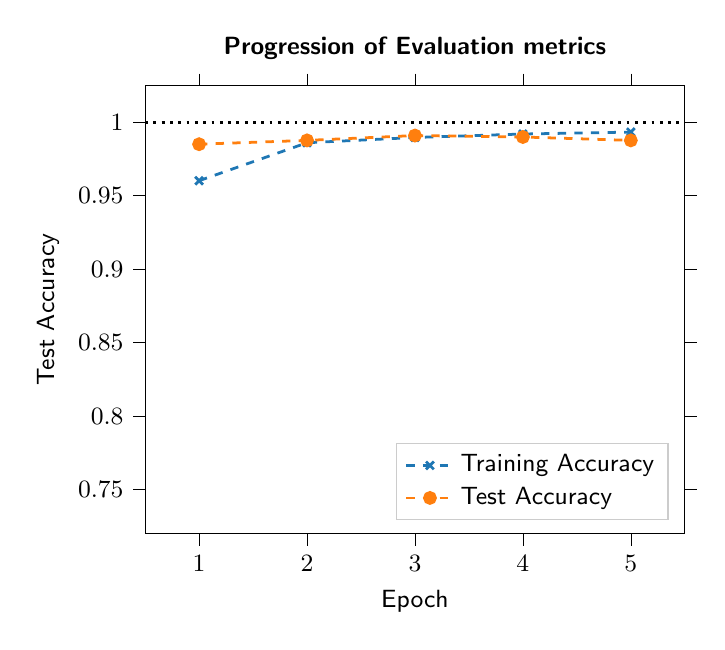
\begin{tikzpicture}

\definecolor{color0}{rgb}{0.12156862745098,0.466666666666667,0.705882352941177}
\definecolor{color1}{rgb}{1,0.498039215686275,0.0549019607843137}

\begin{axis}[
font=\small,
legend cell align={left},
legend style={at={(0.97,0.03)}, anchor=south east, draw=white!80.0!black},
minor xtick={},
minor ytick={},
tick align=outside,
tick pos=both,
title={{\bf Progression of Evaluation metrics}},
x grid style={white!69.01960784313725!black},
xlabel={Epoch},
xmin=0.5, xmax=5.5,
xtick style={color=black},
xtick={1,2,3,4,5},
y grid style={white!69.01960784313725!black},
ylabel={Test Accuracy},
ymin=0.72, ymax=1.025,
ytick style={color=black},
ytick={0.7,0.75,0.8,0.85,0.9,0.95,1,1.05}
]
\addplot [line width=1.0pt, color0, dashed, mark=x, mark size=2, mark options={solid}]
table {%
1 0.960166666666667
2 0.986
3 0.989583333333333
4 0.991933333333333
5 0.99325
};
\addlegendentry{Training Accuracy}
\addplot [line width=1.0pt, color1, dashed, mark=*, mark size=2, mark options={solid}]
table {%
1 0.985
2 0.9876
3 0.9909
4 0.9899
5 0.9876
};
\addlegendentry{Test Accuracy}
\addplot [line width=1.0pt, black, dotted, forget plot]
table {%
0.5 1
5.5 1
};
\end{axis}

\end{tikzpicture}
            \caption{Accuracy learning process for model \protect\hyperref[training:1]
                        {1}.}
        \end{subfigure}%
        \hfill%
        \begin{subfigure}{.5\textwidth}
            % This file was created by tikzplotlib v0.8.2.
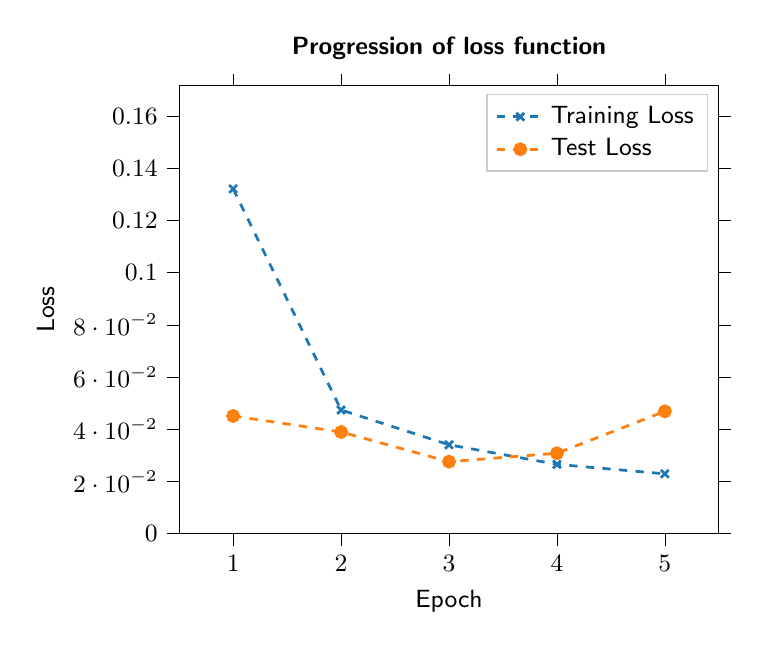
\begin{tikzpicture}

\definecolor{color0}{rgb}{0.12156862745098,0.466666666666667,0.705882352941177}
\definecolor{color1}{rgb}{1,0.498039215686275,0.0549019607843137}

\begin{axis}[
font=\small,
legend cell align={left},
legend style={draw=white!80.0!black},
minor xtick={},
minor ytick={},
tick align=outside,
tick pos=both,
title={{\bf Progression of loss function}},
x grid style={white!69.01960784313725!black},
xlabel={Epoch},
xmin=0.5, xmax=5.5,
xtick style={color=black},
xtick={1,2,3,4,5},
y grid style={white!69.01960784313725!black},
ylabel={Loss},
ymin=0, ymax=0.171749340473488,
ytick style={color=black},
ytick={0,0.02,0.04,0.06,0.08,0.1,0.12,0.14,0.16,0.18}
]
\addplot [line width=1.0pt, color0, dashed, mark=x, mark size=2, mark options={solid}]
table {%
1 0.132114877287298
2 0.0474134801289377
3 0.0340738017865612
4 0.0265769775162839
5 0.0229504140371146
};
\addlegendentry{Training Loss}
\addplot [line width=1.0pt, color1, dashed, mark=*, mark size=2, mark options={solid}]
table {%
1 0.045107334170863
2 0.0389748287099879
3 0.0276051344647305
4 0.0308365761081688
5 0.0468869591456067
};
\addlegendentry{Test Loss}
\end{axis}

\end{tikzpicture}
            \caption{Loss learning process for model \protect\hyperref[training:1]
                        {1}.}
        \end{subfigure}
        \par\bigskip
        \begin{subfigure}{.5\textwidth}
            % This file was created by tikzplotlib v0.8.2.
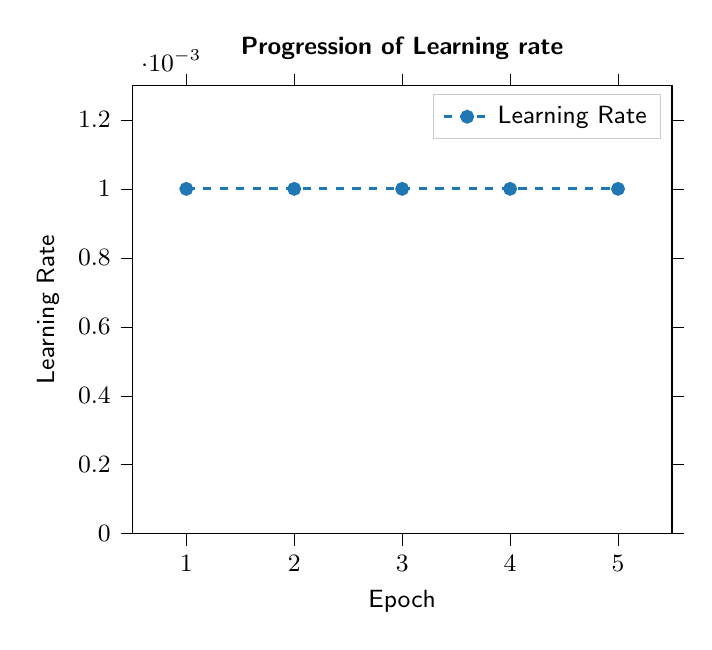
\begin{tikzpicture}

\definecolor{color0}{rgb}{0.12156862745098,0.466666666666667,0.705882352941177}

\begin{axis}[
font=\small,
legend cell align={left},
legend style={draw=white!80.0!black},
minor xtick={},
minor ytick={},
tick align=outside,
tick pos=both,
title={{\bf Progression of Learning rate}},
x grid style={white!69.01960784313725!black},
xlabel={Epoch},
xmin=0.5, xmax=5.5,
xtick style={color=black},
xtick={1,2,3,4,5},
y grid style={white!69.01960784313725!black},
ylabel={Learning Rate},
ymin=0, ymax=0.0013,
ytick style={color=black},
ytick={0,0.0002,0.0004,0.0006,0.0008,0.001,0.0012,0.0014}
]
\addplot [line width=1.0pt, color0, dashed, mark=*, mark size=2, mark options={solid}]
table {%
1 0.001
2 0.001
3 0.001
4 0.001
5 0.001
};
\addlegendentry{Learning Rate}
\end{axis}

\end{tikzpicture}
            \caption{Learning rate per epoch for model \protect\hyperref[training:1]
                        {1}.}
        \end{subfigure}%
        \caption{Training and evaluation metrics for model  \protect\hyperref[training:1]
                    {1}.
                \label{fig:results1}}
    \end{figure}

    \subsubsection*{Dataset}
    \begin{description}
        \item[Name] MNIST
        \item[Train-Test-Dev split:] {\it Training set:}
        60000,
        {\it Test set:}
        10000,
        {\it Dev set:}
        0,
        \item[Image size] [28, 28]


    \end{description}
    %
    \subsubsection*{Training}
    \begin{description}
        \item[Number of epochs] 5
        \item[Optimizer] RMSProp

            \begin{tabular}{rl}
                    {\bf Learning Rate} & 0.00010000000474974513 \\
                    {\bf Rho} & 0.8999999761581421 \\
                    {\bf Decay} & 0.0 \\
                    {\bf Epsilon} & 1e-07 \\
            \end{tabular}

        \item[Loss] Categorical crossentropy
        \item[Batch size] 64
        \item[Shuffle] Yes
        \item[Training time] 52 sec
    \end{description}
    %
    \subsubsection*{Platform}
    \begin{description}
        \item[Weights exported to path] weights\textbackslash ConvNet2layers\_5ep\_MNIST.h5
        \item[Device used] GPU (GeForce GTX 1060 6GB)
        \item[CPU] Intel(R) Xeon(R) CPU E3-1245 v5 @ 3.50GHz,
                   X86\_64
        \item[Python Version] 3.7.2.final.0 (64 bit)
        \item[Keras Version] 2.2.5 (Backend: tensorflow)
        \item[Tensorflow Version] 1.14.0
        \item[Timestamp] 26.09.2019 at 10:07
    \end{description}
    \newpage
    %
    \subsection{Model 2:
                        MLP2layers
                \label{training:2}
                }
    %
    \paragraph*{Training history} See Figure \ref{fig:results2}.
    \begin{figure}[H]
        \centering
        \begin{subfigure}{.5\textwidth}
            % This file was created by tikzplotlib v0.8.2.
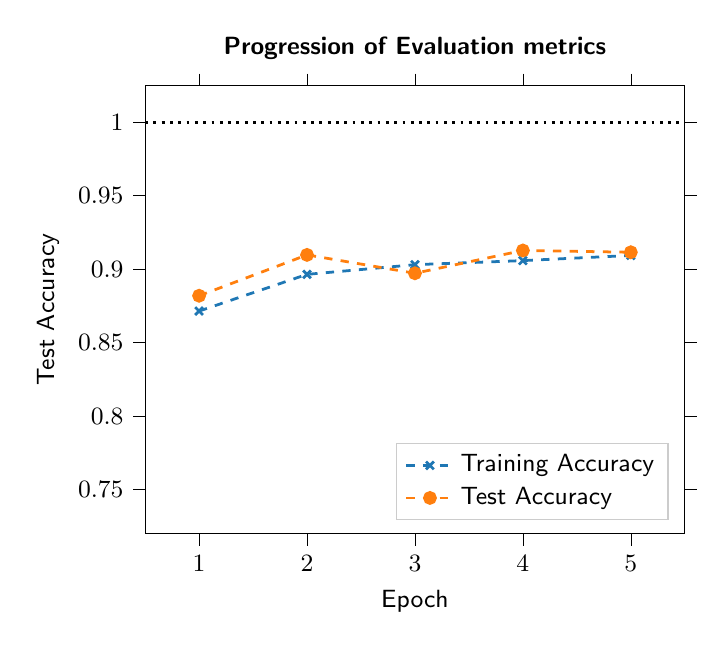
\begin{tikzpicture}

\definecolor{color0}{rgb}{0.12156862745098,0.466666666666667,0.705882352941177}
\definecolor{color1}{rgb}{1,0.498039215686275,0.0549019607843137}

\begin{axis}[
font=\small,
legend cell align={left},
legend style={at={(0.97,0.03)}, anchor=south east, draw=white!80.0!black},
minor xtick={},
minor ytick={},
tick align=outside,
tick pos=both,
title={{\bf Progression of Evaluation metrics}},
x grid style={white!69.01960784313725!black},
xlabel={Epoch},
xmin=0.5, xmax=5.5,
xtick style={color=black},
xtick={1,2,3,4,5},
y grid style={white!69.01960784313725!black},
ylabel={Test Accuracy},
ymin=0.72, ymax=1.025,
ytick style={color=black},
ytick={0.7,0.75,0.8,0.85,0.9,0.95,1,1.05}
]
\addplot [line width=1.0pt, color0, dashed, mark=x, mark size=2, mark options={solid}]
table {%
1 0.871483333333333
2 0.89645
3 0.90305
4 0.905816666666667
5 0.909333333333333
};
\addlegendentry{Training Accuracy}
\addplot [line width=1.0pt, color1, dashed, mark=*, mark size=2, mark options={solid}]
table {%
1 0.8819
2 0.9097
3 0.8972
4 0.9127
5 0.9115
};
\addlegendentry{Test Accuracy}
\addplot [line width=1.0pt, black, dotted, forget plot]
table {%
0.5 1
5.5 1
};
\end{axis}

\end{tikzpicture}
            \caption{Accuracy learning process for model \protect\hyperref[training:2]
                        {2}.}
        \end{subfigure}%
        \hfill%
        \begin{subfigure}{.5\textwidth}
            % This file was created by tikzplotlib v0.8.2.
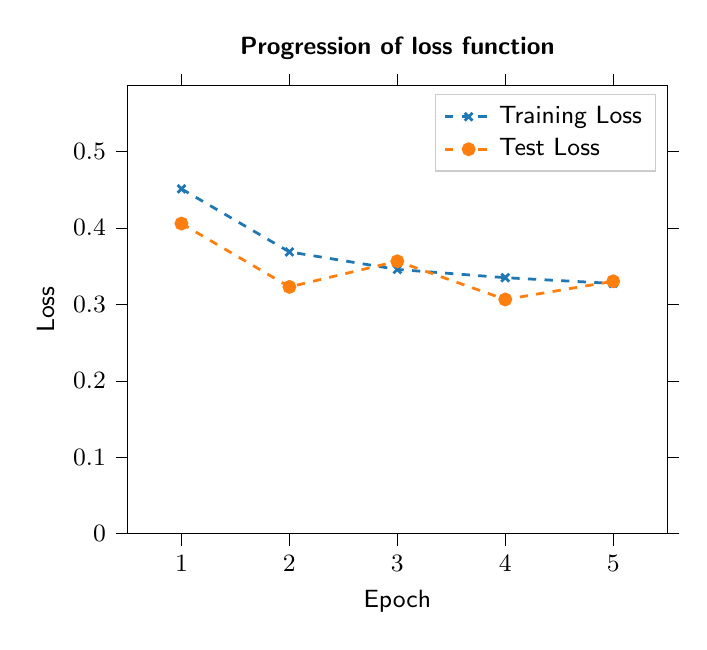
\begin{tikzpicture}

\definecolor{color0}{rgb}{0.12156862745098,0.466666666666667,0.705882352941177}
\definecolor{color1}{rgb}{1,0.498039215686275,0.0549019607843137}

\begin{axis}[
font=\small,
legend cell align={left},
legend style={draw=white!80.0!black},
minor xtick={},
minor ytick={},
tick align=outside,
tick pos=both,
title={{\bf Progression of loss function}},
x grid style={white!69.01960784313725!black},
xlabel={Epoch},
xmin=0.5, xmax=5.5,
xtick style={color=black},
xtick={1,2,3,4,5},
y grid style={white!69.01960784313725!black},
ylabel={Loss},
ymin=0, ymax=0.586448700480461,
ytick style={color=black},
ytick={0,0.1,0.2,0.3,0.4,0.5,0.6}
]
\addplot [line width=1.0pt, color0, dashed, mark=x, mark size=2, mark options={solid}]
table {%
1 0.45111438498497
2 0.36865783469677
3 0.345719545857112
4 0.33494815762043
5 0.327389693391323
};
\addlegendentry{Training Loss}
\addplot [line width=1.0pt, color1, dashed, mark=*, mark size=2, mark options={solid}]
table {%
1 0.405732521235943
2 0.322877946376801
3 0.356435169196129
4 0.30648259422183
5 0.330229531121254
};
\addlegendentry{Test Loss}
\end{axis}

\end{tikzpicture}
            \caption{Loss learning process for model \protect\hyperref[training:2]
                        {2}.}
        \end{subfigure}
        \par\bigskip
        \begin{subfigure}{.5\textwidth}
            % This file was created by tikzplotlib v0.8.2.
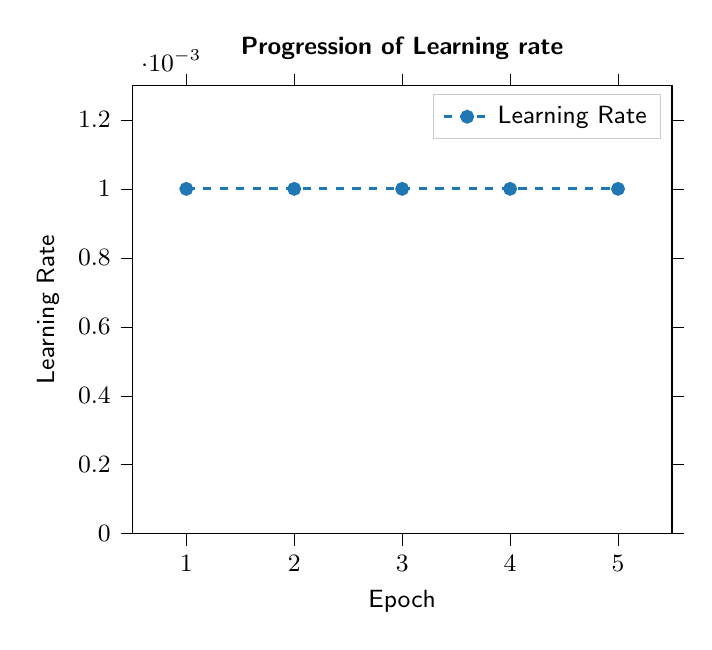
\begin{tikzpicture}

\definecolor{color0}{rgb}{0.12156862745098,0.466666666666667,0.705882352941177}

\begin{axis}[
font=\small,
legend cell align={left},
legend style={draw=white!80.0!black},
minor xtick={},
minor ytick={},
tick align=outside,
tick pos=both,
title={{\bf Progression of Learning rate}},
x grid style={white!69.01960784313725!black},
xlabel={Epoch},
xmin=0.5, xmax=5.5,
xtick style={color=black},
xtick={1,2,3,4,5},
y grid style={white!69.01960784313725!black},
ylabel={Learning Rate},
ymin=0, ymax=0.0013,
ytick style={color=black},
ytick={0,0.0002,0.0004,0.0006,0.0008,0.001,0.0012,0.0014}
]
\addplot [line width=1.0pt, color0, dashed, mark=*, mark size=2, mark options={solid}]
table {%
1 0.001
2 0.001
3 0.001
4 0.001
5 0.001
};
\addlegendentry{Learning Rate}
\end{axis}

\end{tikzpicture}
            \caption{Learning rate per epoch for model \protect\hyperref[training:2]
                        {2}.}
        \end{subfigure}%
        \caption{Training and evaluation metrics for model  \protect\hyperref[training:2]
                    {2}.
                \label{fig:results2}}
    \end{figure}

    \subsubsection*{Dataset}
    \begin{description}
        \item[Name] MNIST
        \item[Train-Test-Dev split:] {\it Training set:}
        60000,
        {\it Test set:}
        10000,
        {\it Dev set:}
        0,
        \item[Image size] [28, 28]


    \end{description}
    %
    \subsubsection*{Training}
    \begin{description}
        \item[Number of epochs] 5
        \item[Optimizer] RMSProp

            \begin{tabular}{rl}
                    {\bf Learning Rate} & 0.0010000000474974513 \\
                    {\bf Rho} & 0.8999999761581421 \\
                    {\bf Decay} & 0.0 \\
                    {\bf Epsilon} & 1e-07 \\
            \end{tabular}

        \item[Loss] Categorical crossentropy
        \item[Batch size] 64
        \item[Shuffle] Yes
        \item[Training time] 29 sec
    \end{description}
    %
    \subsubsection*{Platform}
    \begin{description}
        \item[Weights exported to path] weights\textbackslash MLP2layers\_5ep\_MNIST.h5
        \item[Device used] GPU (GeForce GTX 1060 6GB)
        \item[CPU] Intel(R) Xeon(R) CPU E3-1245 v5 @ 3.50GHz,
                   X86\_64
        \item[Python Version] 3.7.2.final.0 (64 bit)
        \item[Keras Version] 2.2.5 (Backend: tensorflow)
        \item[Tensorflow Version] 1.14.0
        \item[Timestamp] 26.09.2019 at 10:08
    \end{description}
    \newpage
    %
    \subsection{Model 3:
                        MLP5layers
                \label{training:3}
                }
    %
    \paragraph*{Training history} See Figure \ref{fig:results3}.
    \begin{figure}[H]
        \centering
        \begin{subfigure}{.5\textwidth}
            % This file was created by tikzplotlib v0.8.2.
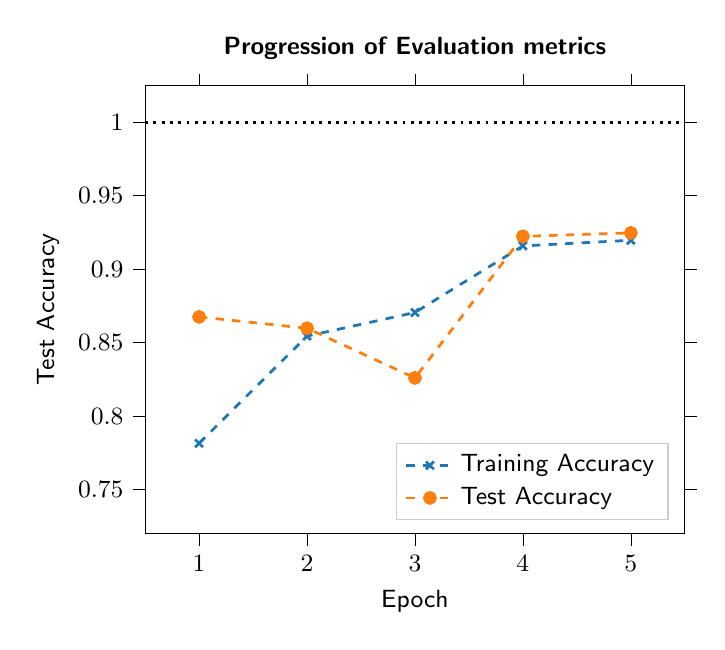
\begin{tikzpicture}

\definecolor{color0}{rgb}{0.12156862745098,0.466666666666667,0.705882352941177}
\definecolor{color1}{rgb}{1,0.498039215686275,0.0549019607843137}

\begin{axis}[
font=\small,
legend cell align={left},
legend style={at={(0.97,0.03)}, anchor=south east, draw=white!80.0!black},
minor xtick={},
minor ytick={},
tick align=outside,
tick pos=both,
title={{\bf Progression of Evaluation metrics}},
x grid style={white!69.01960784313725!black},
xlabel={Epoch},
xmin=0.5, xmax=5.5,
xtick style={color=black},
xtick={1,2,3,4,5},
y grid style={white!69.01960784313725!black},
ylabel={Test Accuracy},
ymin=0.72, ymax=1.025,
ytick style={color=black},
ytick={0.7,0.75,0.8,0.85,0.9,0.95,1,1.05}
]
\addplot [line width=1.0pt, color0, dashed, mark=x, mark size=2, mark options={solid}]
table {%
1 0.781516666666667
2 0.854433333333333
3 0.870516666666667
4 0.915816666666667
5 0.91965
};
\addlegendentry{Training Accuracy}
\addplot [line width=1.0pt, color1, dashed, mark=*, mark size=2, mark options={solid}]
table {%
1 0.8675
2 0.8598
3 0.826
4 0.9223
5 0.9247
};
\addlegendentry{Test Accuracy}
\addplot [line width=1.0pt, black, dotted, forget plot]
table {%
0.5 1
5.5 1
};
\end{axis}

\end{tikzpicture}
            \caption{Accuracy learning process for model \protect\hyperref[training:3]
                        {3}.}
        \end{subfigure}%
        \hfill%
        \begin{subfigure}{.5\textwidth}
            % This file was created by tikzplotlib v0.8.2.
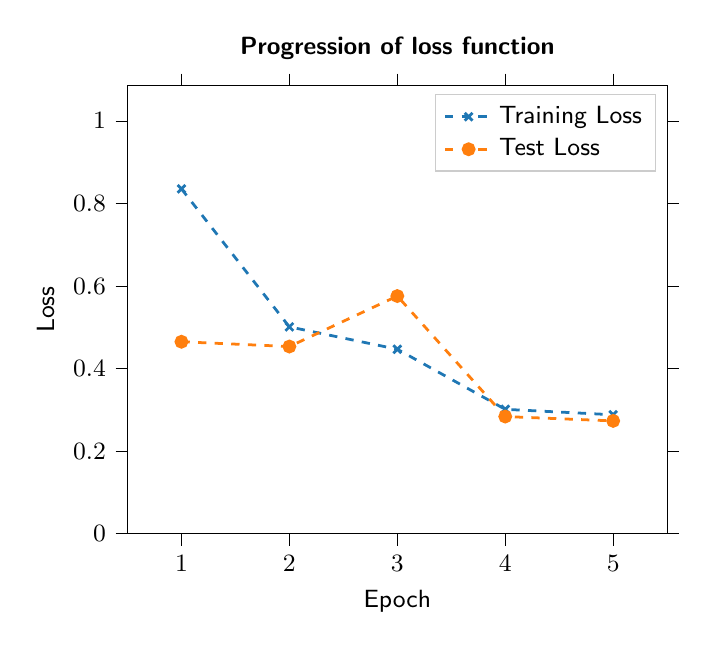
\begin{tikzpicture}

\definecolor{color0}{rgb}{0.12156862745098,0.466666666666667,0.705882352941177}
\definecolor{color1}{rgb}{1,0.498039215686275,0.0549019607843137}

\begin{axis}[
font=\small,
legend cell align={left},
legend style={draw=white!80.0!black},
minor xtick={},
minor ytick={},
tick align=outside,
tick pos=both,
title={{\bf Progression of loss function}},
x grid style={white!69.01960784313725!black},
xlabel={Epoch},
xmin=0.5, xmax=5.5,
xtick style={color=black},
xtick={1,2,3,4,5},
y grid style={white!69.01960784313725!black},
ylabel={Loss},
ymin=0, ymax=1.08574285008748,
ytick style={color=black},
ytick={0,0.2,0.4,0.6,0.8,1,1.2}
]
\addplot [line width=1.0pt, color0, dashed, mark=x, mark size=2, mark options={solid}]
table {%
1 0.835186807759603
2 0.500995210758845
3 0.446815415763855
4 0.30130756948789
5 0.288122650122643
};
\addlegendentry{Training Loss}
\addplot [line width=1.0pt, color1, dashed, mark=*, mark size=2, mark options={solid}]
table {%
1 0.464935952138901
2 0.453388179993629
3 0.575645192313194
4 0.283792906475067
5 0.273271721291542
};
\addlegendentry{Test Loss}
\end{axis}

\end{tikzpicture}
            \caption{Loss learning process for model \protect\hyperref[training:3]
                        {3}.}
        \end{subfigure}
        \par\bigskip
        \begin{subfigure}{.5\textwidth}
            % This file was created by tikzplotlib v0.8.2.
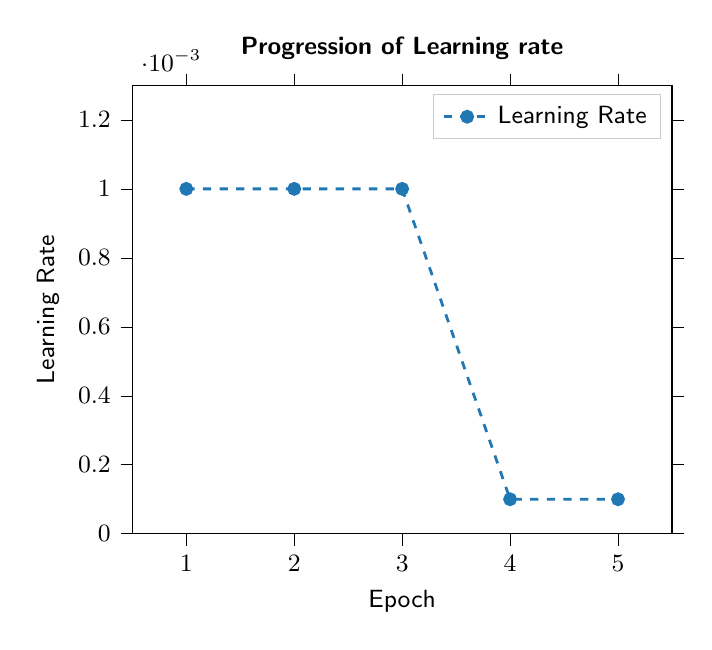
\begin{tikzpicture}

\definecolor{color0}{rgb}{0.12156862745098,0.466666666666667,0.705882352941177}

\begin{axis}[
font=\small,
legend cell align={left},
legend style={draw=white!80.0!black},
minor xtick={},
minor ytick={},
tick align=outside,
tick pos=both,
title={{\bf Progression of Learning rate}},
x grid style={white!69.01960784313725!black},
xlabel={Epoch},
xmin=0.5, xmax=5.5,
xtick style={color=black},
xtick={1,2,3,4,5},
y grid style={white!69.01960784313725!black},
ylabel={Learning Rate},
ymin=0, ymax=0.0013,
ytick style={color=black},
ytick={0,0.0002,0.0004,0.0006,0.0008,0.001,0.0012,0.0014}
]
\addplot [line width=1.0pt, color0, dashed, mark=*, mark size=2, mark options={solid}]
table {%
1 0.001
2 0.001
3 0.001
4 0.000100000005
5 0.000100000005
};
\addlegendentry{Learning Rate}
\end{axis}

\end{tikzpicture}
            \caption{Learning rate per epoch for model \protect\hyperref[training:3]
                        {3}.}
        \end{subfigure}%
        \caption{Training and evaluation metrics for model  \protect\hyperref[training:3]
                    {3}.
                \label{fig:results3}}
    \end{figure}

    \subsubsection*{Dataset}
    \begin{description}
        \item[Name] MNIST
        \item[Train-Test-Dev split:] {\it Training set:}
        60000,
        {\it Test set:}
        10000,
        {\it Dev set:}
        0,
        \item[Image size] [28, 28]


    \end{description}
    %
    \subsubsection*{Training}
    \begin{description}
        \item[Number of epochs] 5
        \item[Optimizer] RMSProp

            \begin{tabular}{rl}
                    {\bf Learning Rate} & 0.00010000000474974513 \\
                    {\bf Rho} & 0.8999999761581421 \\
                    {\bf Decay} & 0.0 \\
                    {\bf Epsilon} & 1e-07 \\
            \end{tabular}

        \item[Loss] Categorical crossentropy
        \item[Batch size] 64
        \item[Shuffle] Yes
        \item[Training time] 39 sec
    \end{description}
    %
    \subsubsection*{Platform}
    \begin{description}
        \item[Weights exported to path] weights\textbackslash MLP5layers\_5ep\_MNIST.h5
        \item[Device used] GPU (GeForce GTX 1060 6GB)
        \item[CPU] Intel(R) Xeon(R) CPU E3-1245 v5 @ 3.50GHz,
                   X86\_64
        \item[Python Version] 3.7.2.final.0 (64 bit)
        \item[Keras Version] 2.2.5 (Backend: tensorflow)
        \item[Tensorflow Version] 1.14.0
        \item[Timestamp] 26.09.2019 at 10:09
    \end{description}
    \newpage
% %%%%%%%%%%%%%%%%%%%%%%%%%%%%%%%%%%%%%%%%%%%%%%%%%%%%%%%%%%%%%%%%%%%

% %%%%%%%%%%%%%%%%%%%%%%%%%%%%%%%%%%%%%%%%%%%%%%%%%%%%%%%%%%%%%%%%%%%
\section{Model Architectures}
\subsection{ConvNet2layers
            \label{model:ConvNet2layers}
            }
\paragraph{Used in \No{}:}
    \hyperref[training:3]
             {3}
\vspace{-2ex}
%
\paragraph{Model summary:}$\,$\\
\begin{longtable}{rR{.22\textwidth}cL{.22\textwidth}rL{.22\textwidth}}
    \hline\\[-1.5ex]
    \No{} &
    Layer (Type) &
    Output shape &
    Config &
    \#Parameters &
    Inbound layers\\
    \hline\\
    \endhead
        0
        &
        \color{InputLayer}{
        input\_1}
        \color{InputLayer}{
        (InputLayer)}
        &
        (28, 28, 1)
        &
        &
        \num{0}
        &
        \\
        \hline\\[-1.5ex]
        1
        &
        \color{Conv2D}{
        conv2d\_1}
        \color{Conv2D}{
        (Conv2D)}
        &
        (26, 26, 32)
        &
            {\bf Activation:} relu \newline
            {\bf Kernel Size:} [3, 3] \newline
            {\bf Stride:} [1, 1] \newline
            {\bf Dilation:} [1, 1] \newline
            {\bf Padding:} valid
        &
        \num{320}
        &
        \color{InputLayer}{
            input\_1}
        \\
        \hline\\[-1.5ex]
        2
        &
        \color{Conv2D}{
        conv2d\_2}
        \color{Conv2D}{
        (Conv2D)}
        &
        (24, 24, 64)
        &
            {\bf Activation:} relu \newline
            {\bf Kernel Size:} [3, 3] \newline
            {\bf Stride:} [1, 1] \newline
            {\bf Dilation:} [1, 1] \newline
            {\bf Padding:} valid
        &
        \num{18496}
        &
        \color{Conv2D}{
            conv2d\_1}
        \\
        \hline\\[-1.5ex]
        3
        &
        \color{MaxPooling2D}{
        max\_pooling2d\_1}
        \color{MaxPooling2D}{
        (MaxPooling2D)}
        &
        (12, 12, 64)
        &
            {\bf Pool size:} [2, 2] \newline
            {\bf Strides:} [2, 2] \newline
            {\bf Padding:} valid
        &
        \num{0}
        &
        \color{Conv2D}{
            conv2d\_2}
        \\
        \hline\\[-1.5ex]
        4
        &
        \color{Dropout}{
        dropout\_1}
        \color{Dropout}{
        (Dropout)}
        &
        (12, 12, 64)
        &
            {\bf Dropout Rate:} 0.0
        &
        \num{0}
        &
        \color{MaxPooling2D}{
            max\_pooling2d\_1}
        \\
        \hline\\[-1.5ex]
        5
        &
        \color{Flatten}{
        flatten\_1}
        \color{Flatten}{
        (Flatten)}
        &
        (9216,)
        &
        &
        \num{0}
        &
        \color{Dropout}{
            dropout\_1}
        \\
        \hline\\[-1.5ex]
        6
        &
        \color{Dense}{
        dense\_1}
        \color{Dense}{
        (Dense)}
        &
        (128,)
        &
            {\bf \#Neurons:} 128\newline
            {\bf Activation:} relu
        &
        \num{1179776}
        &
        \color{Flatten}{
            flatten\_1}
        \\
        \hline\\[-1.5ex]
        7
        &
        \color{Dropout}{
        dropout\_2}
        \color{Dropout}{
        (Dropout)}
        &
        (128,)
        &
            {\bf Dropout Rate:} 0.2
        &
        \num{0}
        &
        \color{Dense}{
            dense\_1}
        \\
        \hline\\[-1.5ex]
        8
        &
        \color{Dense}{
        dense\_2}
        \color{Dense}{
        (Dense)}
        &
        (10,)
        &
            {\bf \#Neurons:} 10\newline
            {\bf Activation:} softmax
        &
        \num{1290}
        &
        \color{Dropout}{
            dropout\_2}
        \\
        \hline\\[-1.5ex]
\end{longtable}
\newpage
\subsection{MLP5layers
            \label{model:MLP5layers}
            }
\paragraph{Used in \No{}:}
    \hyperref[training:3]
             {3}
\vspace{-2ex}
%
\paragraph{Model summary:}$\,$\\
\begin{longtable}{rR{.22\textwidth}cL{.22\textwidth}rL{.22\textwidth}}
    \hline\\[-1.5ex]
    \No{} &
    Layer (Type) &
    Output shape &
    Config &
    \#Parameters &
    Inbound layers\\
    \hline\\
    \endhead
        0
        &
        \color{InputLayer}{
        input\_3}
        \color{InputLayer}{
        (InputLayer)}
        &
        (28, 28, 1)
        &
        &
        \num{0}
        &
        \\
        \hline\\[-1.5ex]
        1
        &
        \color{Flatten}{
        flatten\_3}
        \color{Flatten}{
        (Flatten)}
        &
        (784,)
        &
        &
        \num{0}
        &
        \color{InputLayer}{
            input\_3}
        \\
        \hline\\[-1.5ex]
        2
        &
        \color{Dense}{
        dense\_6}
        \color{Dense}{
        (Dense)}
        &
        (512,)
        &
            {\bf \#Neurons:} 512\newline
            {\bf Activation:} linear
        &
        \num{401920}
        &
        \color{Flatten}{
            flatten\_3}
        \\
        \hline\\[-1.5ex]
        3
        &
        \color{Dropout}{
        dropout\_5}
        \color{Dropout}{
        (Dropout)}
        &
        (512,)
        &
            {\bf Dropout Rate:} 0.0
        &
        \num{0}
        &
        \color{Dense}{
            dense\_6}
        \\
        \hline\\[-1.5ex]
        4
        &
        \color{Dense}{
        dense\_7}
        \color{Dense}{
        (Dense)}
        &
        (512,)
        &
            {\bf \#Neurons:} 512\newline
            {\bf Activation:} linear
        &
        \num{262656}
        &
        \color{Dropout}{
            dropout\_5}
        \\
        \hline\\[-1.5ex]
        5
        &
        \color{Dropout}{
        dropout\_6}
        \color{Dropout}{
        (Dropout)}
        &
        (512,)
        &
            {\bf Dropout Rate:} 0.0
        &
        \num{0}
        &
        \color{Dense}{
            dense\_7}
        \\
        \hline\\[-1.5ex]
        6
        &
        \color{Dense}{
        dense\_8}
        \color{Dense}{
        (Dense)}
        &
        (512,)
        &
            {\bf \#Neurons:} 512\newline
            {\bf Activation:} linear
        &
        \num{262656}
        &
        \color{Dropout}{
            dropout\_6}
        \\
        \hline\\[-1.5ex]
        7
        &
        \color{Dropout}{
        dropout\_7}
        \color{Dropout}{
        (Dropout)}
        &
        (512,)
        &
            {\bf Dropout Rate:} 0.0
        &
        \num{0}
        &
        \color{Dense}{
            dense\_8}
        \\
        \hline\\[-1.5ex]
        8
        &
        \color{Dense}{
        dense\_9}
        \color{Dense}{
        (Dense)}
        &
        (512,)
        &
            {\bf \#Neurons:} 512\newline
            {\bf Activation:} linear
        &
        \num{262656}
        &
        \color{Dropout}{
            dropout\_7}
        \\
        \hline\\[-1.5ex]
        9
        &
        \color{Dropout}{
        dropout\_8}
        \color{Dropout}{
        (Dropout)}
        &
        (512,)
        &
            {\bf Dropout Rate:} 0.2
        &
        \num{0}
        &
        \color{Dense}{
            dense\_9}
        \\
        \hline\\[-1.5ex]
        10
        &
        \color{Dense}{
        dense\_10}
        \color{Dense}{
        (Dense)}
        &
        (512,)
        &
            {\bf \#Neurons:} 512\newline
            {\bf Activation:} linear
        &
        \num{262656}
        &
        \color{Dropout}{
            dropout\_8}
        \\
        \hline\\[-1.5ex]
        11
        &
        \color{Dropout}{
        dropout\_9}
        \color{Dropout}{
        (Dropout)}
        &
        (512,)
        &
            {\bf Dropout Rate:} 0.2
        &
        \num{0}
        &
        \color{Dense}{
            dense\_10}
        \\
        \hline\\[-1.5ex]
        12
        &
        \color{Dense}{
        dense\_11}
        \color{Dense}{
        (Dense)}
        &
        (10,)
        &
            {\bf \#Neurons:} 10\newline
            {\bf Activation:} softmax
        &
        \num{5130}
        &
        \color{Dropout}{
            dropout\_9}
        \\
        \hline\\[-1.5ex]
\end{longtable}
\newpage
\subsection{MLP2layers
            \label{model:MLP2layers}
            }
\paragraph{Used in \No{}:}
    \hyperref[training:3]
             {3}
\vspace{-2ex}
%
\paragraph{Model summary:}$\,$\\
\begin{longtable}{rR{.22\textwidth}cL{.22\textwidth}rL{.22\textwidth}}
    \hline\\[-1.5ex]
    \No{} &
    Layer (Type) &
    Output shape &
    Config &
    \#Parameters &
    Inbound layers\\
    \hline\\
    \endhead
        0
        &
        \color{InputLayer}{
        input\_2}
        \color{InputLayer}{
        (InputLayer)}
        &
        (28, 28, 1)
        &
        &
        \num{0}
        &
        \\
        \hline\\[-1.5ex]
        1
        &
        \color{Flatten}{
        flatten\_2}
        \color{Flatten}{
        (Flatten)}
        &
        (784,)
        &
        &
        \num{0}
        &
        \color{InputLayer}{
            input\_2}
        \\
        \hline\\[-1.5ex]
        2
        &
        \color{Dense}{
        dense\_3}
        \color{Dense}{
        (Dense)}
        &
        (512,)
        &
            {\bf \#Neurons:} 512\newline
            {\bf Activation:} linear
        &
        \num{401920}
        &
        \color{Flatten}{
            flatten\_2}
        \\
        \hline\\[-1.5ex]
        3
        &
        \color{Dropout}{
        dropout\_3}
        \color{Dropout}{
        (Dropout)}
        &
        (512,)
        &
            {\bf Dropout Rate:} 0.0
        &
        \num{0}
        &
        \color{Dense}{
            dense\_3}
        \\
        \hline\\[-1.5ex]
        4
        &
        \color{Dense}{
        dense\_4}
        \color{Dense}{
        (Dense)}
        &
        (512,)
        &
            {\bf \#Neurons:} 512\newline
            {\bf Activation:} linear
        &
        \num{262656}
        &
        \color{Dropout}{
            dropout\_3}
        \\
        \hline\\[-1.5ex]
        5
        &
        \color{Dropout}{
        dropout\_4}
        \color{Dropout}{
        (Dropout)}
        &
        (512,)
        &
            {\bf Dropout Rate:} 0.2
        &
        \num{0}
        &
        \color{Dense}{
            dense\_4}
        \\
        \hline\\[-1.5ex]
        6
        &
        \color{Dense}{
        dense\_5}
        \color{Dense}{
        (Dense)}
        &
        (10,)
        &
            {\bf \#Neurons:} 10\newline
            {\bf Activation:} softmax
        &
        \num{5130}
        &
        \color{Dropout}{
            dropout\_4}
        \\
        \hline\\[-1.5ex]
\end{longtable}
\newpage
% %%%%%%%%%%%%%%%%%%%%%%%%%%%%%%%%%%%%%%%%%%%%%%%%%%%%%%%%%%%%%%%%%%%

\end{document}